\documentclass[11pt, a4paper]{article}

\usepackage[utf8]{inputenc}
\usepackage{float}
\usepackage{amsmath}
\usepackage[]{biblatex} % References
\usepackage{booktabs} % Tables
\usepackage{siunitx} % Typeset units
\usepackage{graphicx} % Import graphics

\graphicspath{{graphics/}}

\sisetup{per-mode=symbol} % (siunitx) Use symbols for 'per' values e.g. m/s
\DeclareSIUnit\feet{ft} % Add the imperial 'feet' unit
\newcommand{\hPa}{\hecto\pascal} % Shorter command for hPa

\bibliography{refs.bib}

\title{Demonstration Resources}
\author{Christopher Lane}

\begin{document}

\subsection*{Hardware Capabilities}
\begin{table}[H]
    \centering
    \begin{tabular}{@{}lll@{}}
        \toprule
        Phone Hardware & Frequency & Accuracy \\ \midrule
        Barometer & \SI{182}{\hertz} & \SI{\pm1}{\metre} \\
        GNSS & \SI{19}{\mega\hertz} & \begin{tabular}[c]{@{}l@{}} \SIrange{1}{4}{\metre} horizontal\\ \SIrange{2.5}{10}{\metre} vertical\end{tabular}
    \end{tabular}
    \caption{Phone hardware capabilities from~\textcite{kaplan_understanding_2005}}\label{my-label}
\end{table}

\subsubsection*{Initial Altitude Detection Tests}
\begin{figure}[H]
    \centering
    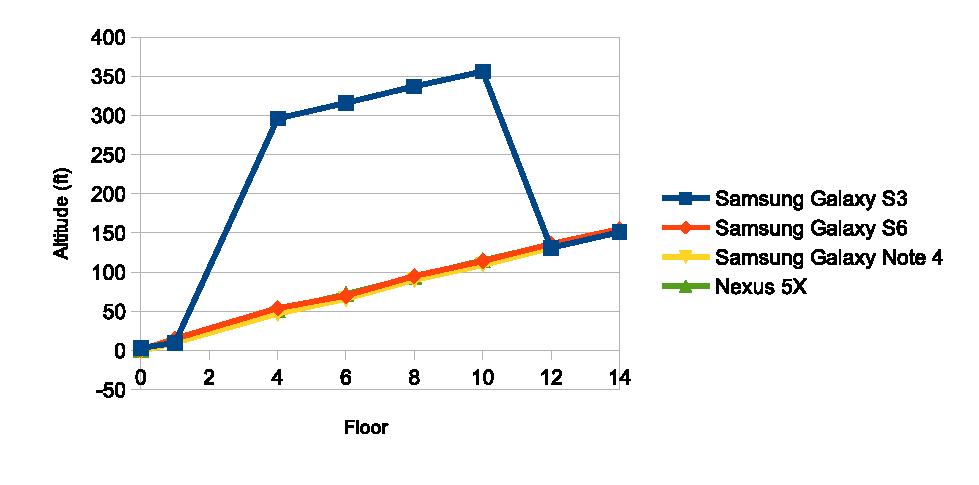
\includegraphics[width=\textwidth]{alt-test-altitude}
    \caption{Altitude measurements from smartphones in Muirhead Tower}\label{fig:alt-test-altitude}
\end{figure}

\begin{figure}[H]
    \centering
    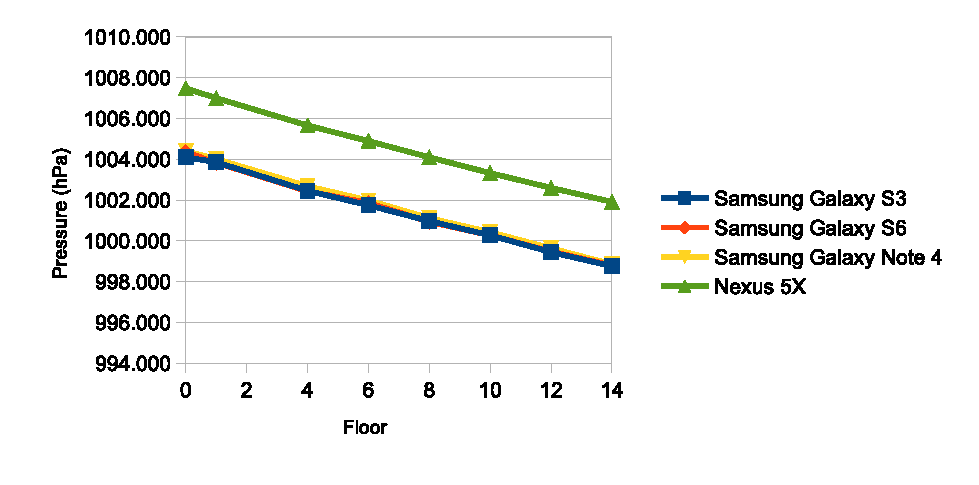
\includegraphics[width=\textwidth]{alt-test-pressure}
    \caption{Air pressure measurements from smartphones in Muirhead Tower}\label{fig:alt-test-pressure}
\end{figure}

\subsubsection*{Landing Pattern Calculations}
\begin{equation}
    Descent Rate = \frac{Air Speed}{Glide Ratio}
\end{equation}

\begin{equation}
    Time Till Altitude = \frac{\delta Altitude}{Descent Rate}
\end{equation}

\begin{equation}
    Distance Travellable = Ground Speed \cdot Time Till Altitude
\end{equation}

\iffalse
    \begin{equation}
        LatAfterMove = \arcsin\left({\sin{Lat} \times \cos{\frac{Distance}{EarthRadius}} \plus \cos{Lat} \times \sin{\frac{Distance}{EarthRadius}} \times \cos{Bearing}}\right)
    \end{equation}
\fi

\begin{multline}
    LatAfterMove = \arcsin\Bigg(\sin{\left( Lat \right)} \cdot \cos{\left(\frac{Distance}{EarthRadius}\right)} \\
    + \cos{\left( Lat \right)} \cdot \sin{\left( \frac{Distance}{EarthRadius} \right)} \cdot \cos{\left( Bearing \right)}\Bigg)
\end{multline}

\subsubsection*{Replay Calculation}
\[
    \begin{pmatrix}
        newX \\ newY
    \end{pmatrix}
    =
    \begin{pmatrix}
        \cos\theta & \sin\theta \\ -\sin\theta & \cos\theta
    \end{pmatrix}
    \begin{pmatrix}
        x \\ y
    \end{pmatrix}
\]

\newpage
\printbibliography{}
\end{document}
